\documentclass[margin=5mm]{standalone}
\usepackage[dvipsnames]{xcolor}
\usepackage{pgfplots}
\usepackage{tikz}
\usepackage[tikz]{ocgx2}

\pgfplotsset{compat=1.18}
\begin{document}

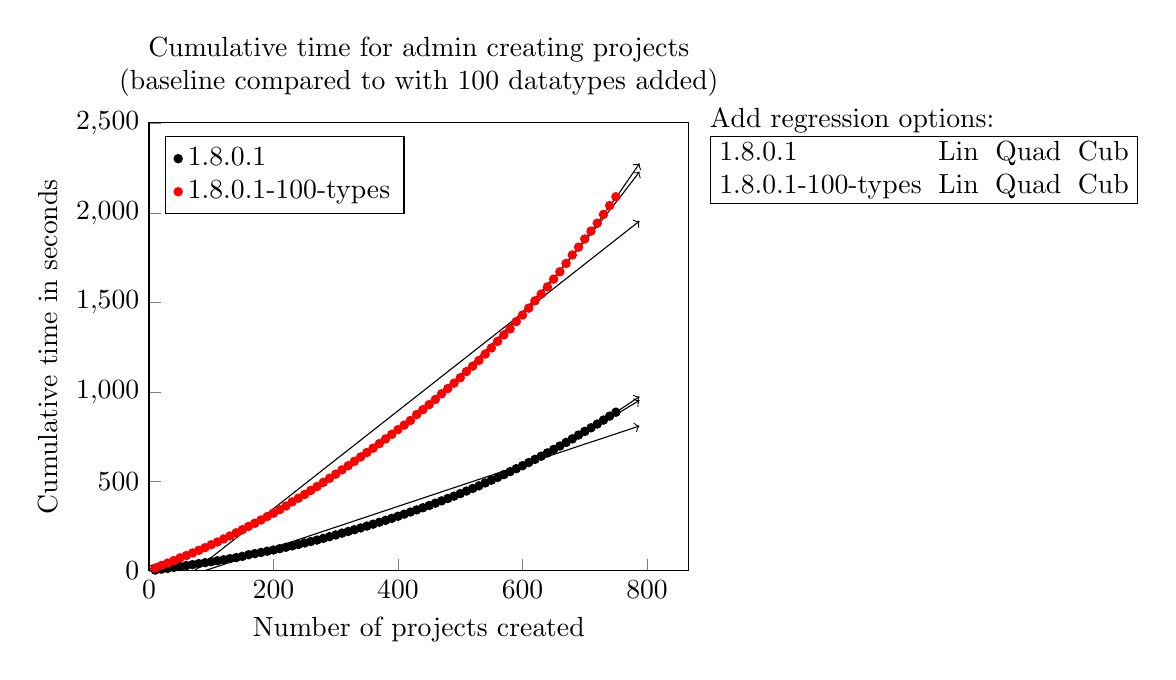
\begin{tikzpicture}
    \begin{axis}[
        align = center,
        legend pos = north west,
        legend cell align = left,
        xlabel = Number of projects created,
        ylabel = Cumulative time in seconds,
        xtick pos = left,
        ytick pos = left,
        scaled ticks = false,
        xmin = 0,
        ymin = 0,
        title = {Cumulative time for admin creating projects (baseline compared to with 100 datatypes added)},
        title style = {text width = 0.8\textwidth},
        legend entries={\switchocg{1.8.0.1}{1.8.0.1},\switchocg{1.8.0.1-100-types}{1.8.0.1-100-types}}]
        \begin{scope}[ocg = {ref = 1.8.0.1-Lin, status = invisible}]
            \plot[domain=0:788,->,forget plot] (\x,{-102.537299099098845545086078345775604248046875 + 1.1581919800853481827829227768233977258205413818359375*(\x)^1});
        \end{scope}
        \begin{scope}[ocg = {ref = 1.8.0.1-Quad, status = invisible}]
            \plot[domain=0:788,->,forget plot] (\x,{13.9420496112552338985324240638874471187591552734375 + 0.25056069143323778103393806304666213691234588623046875*(\x)^1 + 0.00119425169559488259830859480103981695719994604587554931640625*(\x)^2});
        \end{scope}
        \begin{scope}[ocg = {ref = 1.8.0.1-Cub, status = invisible}]
            \plot[domain=0:788,->,forget plot] (\x,{-0.6566972734375442488641283489414490759372711181640625 + 0.473711174204586249469883796336944214999675750732421875*(\x)^1 + 0.00046504355949633971976930890690482556237839162349700927734375*(\x)^2 + 0.000000639656259735564291875786931129699297571278293617069721221923828125*(\x)^3});
        \end{scope}
        \begin{scope}[ocg = {ref = 1.8.0.1, status = visible}]
            \addplot[
                only marks,
                color = black,
                mark = *,
                mark size = 1.5 pt
            ]coordinates {(10,5.132)(20,9.973)(30,14.491)(40,19.84)(50,24.858)(60,29.986)(70,35.315)(80,40.752)(90,46.231)(100,51.713)(110,57.068)(120,62.396)(130,68.928)(140,74.591)(150,81.337)(160,90.521)(170,96.627)(180,103.307)(190,110.129)(200,116.987)(210,124.418)(220,132.295)(230,139.996)(240,147.916)(250,156.223)(260,164.315)(270,172.582)(280,181.816)(290,191.425)(300,200.882)(310,211.253)(320,220.632)(330,230.255)(340,240.131)(350,250.582)(360,261.321)(370,272.124)(380,282.753)(390,293.863)(400,305.524)(410,317.278)(420,329.125)(430,340.93)(440,352.932)(450,365.482)(460,378.413)(470,391.564)(480,404.73)(490,417.859)(500,431.858)(510,446.324)(520,460.557)(530,475.37)(540,491.316)(550,507.065)(560,522.3)(570,538.094)(580,554.56)(590,571.028)(600,587.746)(610,605.379)(620,623.074)(630,640.782)(640,659.534)(650,678.589)(660,697.811)(670,717.808)(680,737.624)(690,759.123)(700,779.198)(710,799.523)(720,820.679)(730,842.541)(740,864.811)(750,886.679)};
        \end{scope}
        \begin{scope}[ocg = {ref = 1.8.0.1-100-types-Lin, status = invisible}]
            \plot[domain=0:788,->,forget plot] (\x,{-198.389056216216459915813175030052661895751953125 + 2.732262147937411622677927880431525409221649169921875*(\x)^1});
        \end{scope}
        \begin{scope}[ocg = {ref = 1.8.0.1-100-types-Quad, status = invisible}]
            \plot[domain=0:788,->,forget plot] (\x,{26.1300430062934907482485868968069553375244140625 + 0.98276267347629475690240496987826190888881683349609375*(\x)^1 + 0.0023019729927119965927351241674614357179962098598480224609375*(\x)^2});
        \end{scope}
        \begin{scope}[ocg = {ref = 1.8.0.1-100-types-Cub, status = invisible}]
            \plot[domain=0:788,->,forget plot] (\x,{-5.58636368258695892308196562225930392742156982421875 + 1.467566713185834981203470306354574859142303466796875*(\x)^1 + 0.00071773689436630872841293982133947793045081198215484619140625*(\x)^2 + 0.000001389680788022533604398668118096171752995360293425619602203369140625*(\x)^3});
        \end{scope}
        \begin{scope}[ocg = {ref = 1.8.0.1-100-types, status = visible}]
            \addplot[
                only marks,
                color = red,
                mark = *,
                mark size = 1.5 pt
            ]coordinates {(10,16.302)(20,30.758)(30,43.892)(40,58.09)(50,72.955)(60,86.309)(70,100.313)(80,114.934)(90,130.115)(100,146.439)(110,161.643)(120,178.902)(130,195.219)(140,212.994)(150,230.568)(160,248.542)(170,266.45)(180,284.878)(190,304.083)(200,323.027)(210,342.264)(220,362.646)(230,385.623)(240,406.687)(250,427.292)(260,449.794)(270,471.464)(280,494.575)(290,517.582)(300,540.913)(310,564.444)(320,587.875)(330,612.346)(340,636.791)(350,661.419)(360,685.97)(370,711.128)(380,737.209)(390,762.802)(400,789.452)(410,814.739)(420,840.853)(430,873.536)(440,900.915)(450,928.949)(460,957.822)(470,989.535)(480,1018.664)(490,1048.798)(500,1079.131)(510,1113.787)(520,1144.029)(530,1175.881)(540,1211.189)(550,1245.316)(560,1282.34)(570,1318.008)(580,1352.142)(590,1393.009)(600,1429.277)(610,1468.007)(620,1508.681)(630,1546.493)(640,1586.551)(650,1629.81)(660,1670.925)(670,1717.394)(680,1764.759)(690,1808.575)(700,1854.146)(710,1898.226)(720,1942.191)(730,1991.183)(740,2040.673)(750,2090.069)};
        \end{scope}
    \end{axis}
    \begin{scope}
        \addtolength{\tabcolsep}{-0.3em}
        \node [below right, shape=rectangle, align=left](regressiontable) at (7,6) {
            Add regression options: \\
            \begin{tabular}{|llll|}
                \hline
                1.8.0.1 & \switchocg{1.8.0.1-Lin}{Lin} & \switchocg{1.8.0.1-Quad}{Quad} & \switchocg{1.8.0.1-Cub}{Cub} \\
                1.8.0.1-100-types & \switchocg{1.8.0.1-100-types-Lin}{Lin} & \switchocg{1.8.0.1-100-types-Quad}{Quad} & \switchocg{1.8.0.1-100-types-Cub}{Cub} \\
                \hline
            \end{tabular}
        };
    \end{scope}
\end{tikzpicture}

\end{document}